
\section{Interpretación de las presentaciones VOR}

Tres componentes del indicador VOR, trabajando conjuntamente, dan al piloto una línea de situación con respecto a la estación de tierra o a cualquier ruta seleccionada en el equipo de a bordo. Estos tres elementos son el selector de rutas OBS, e1 CDI y el indicador o bandera TO-FROM. Al contrario que una aguja de ADF que apunta continuamente a la estación, estos tres componentes no se ven afectados por el rumbo del avión para una posición dada. En consecuencia, el avión y, por tanto, el girodíreccíonal, deben ser orientados según la presentación VOR para obtener una indicación correcta de la dirección de la ruta. Por ello, el piloto deberá efectuar una serie de procedimientos que le permitan acercarse o alejarse de una estación sin posibles errores.

\begin{figure}[htb]
  \centering
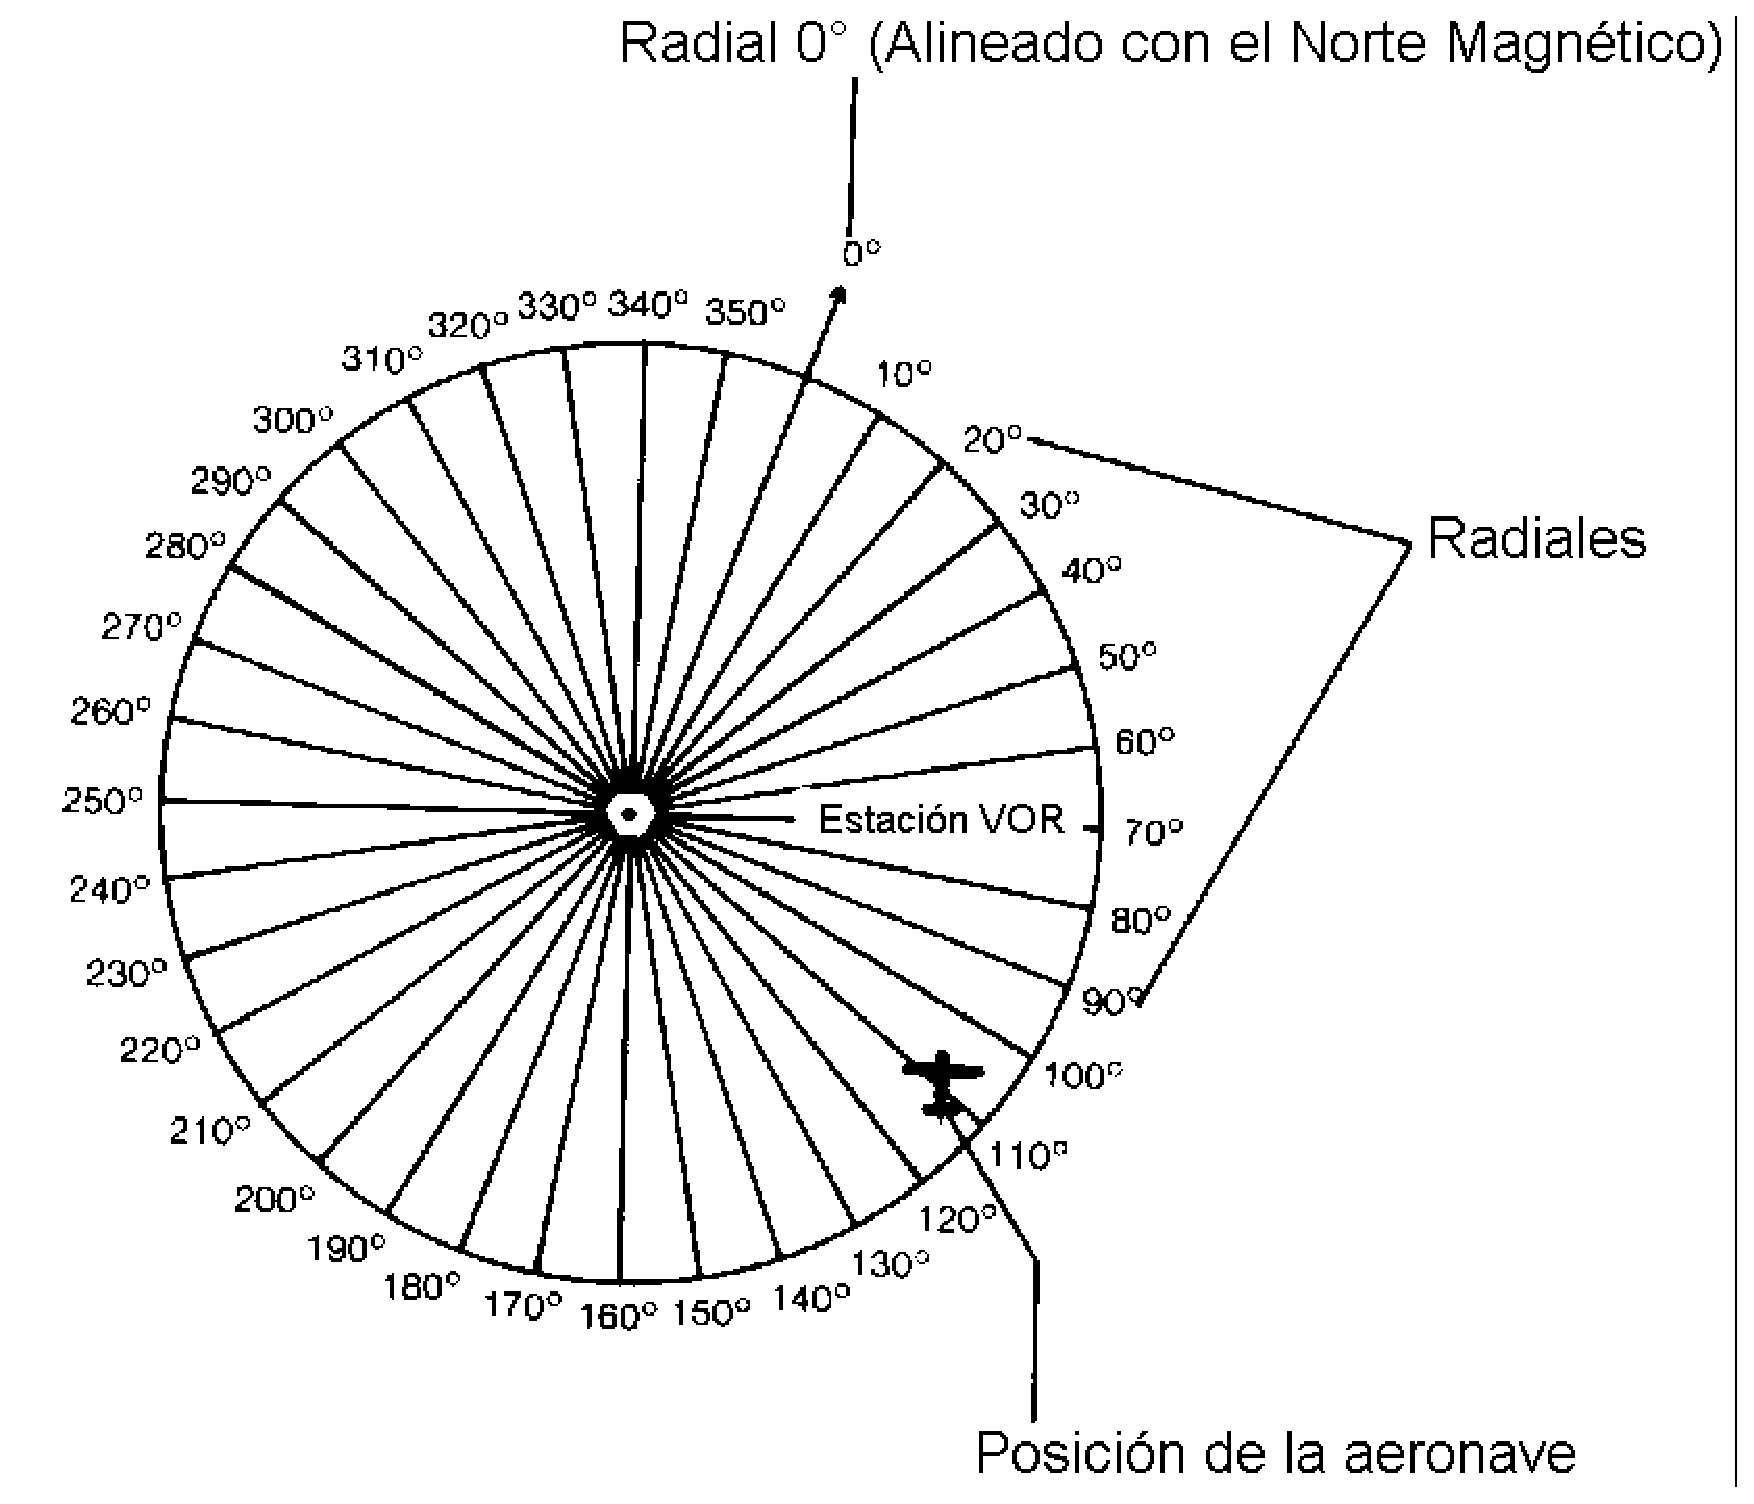
\includegraphics[keepaspectratio,width=0.8\textwidth]{Imagenes/06.02.vor.imagenes/radiales-vor.eps}
  \caption{Radiales de una estación VOR}
  \label{fig:radiales-vor}
\end{figure}


Si el piloto, desde un punto cualquiera, desea dirigirse a una estación VOR, selectará su frecuencia y la identificará. Con el OBS girará la rosa del indicador VOR de a bordo hasta que el CDI quede centrado y aparezca en la ventanilla la bandera con la palabra TO. Cuando esto suceda, mírará debajo del fiel para conocer cuál es su ruta magnética de acercamiento (TO) a la estación. Hará virar su avión hasta que su rumbo magnético coincida con la ruta magnética que señala el fiel del VOR. En el viraje, el CDI, probablemente y dependiendo de la distancia a la estación, habrá sufrido un pequeño desplazamiento, por lo que e1 piloto volverá a centrarlo de nuevo siempre en TO, y tomará el nuevo rumbo magnético que coincida con la Ruta magnética que señale ahora el fiel de indicador VOR. Manteniendo el CDI centrado en esta posición, indudablemente, el avión procederá en arribada a la estación. 

La marcación magnética o QDR del avión con respecto a 1a estación, será la recíproca a la ruta magnética que lleve el avión en ese momento. Si la aeronave prosigue acercándose a la estación, llegará un punto en el que penetre en su cono de silencio. El tiempo que permanezca en él dependerá, lógicamente, de la velocidad y altitud a las que vuele el avión. En ese punto, el CDI oscilará debido a que el instrumento no recibe ningún tipo de señal desde tierra, apareciendo casi simultáneamente la banderilla OFF en ventanilla. Al atravesar el cono de silencio, y suponiendo que el avión haya mantenido constante su rumbo magnético, la bandera OFF se ocultará, apareciendo en su lugar la palabra FROM, y el CDI volverá a centrarse. A partir de esta punta, el piloto sabrá positivamente que ha sobrevolado la estación y que ya se está alejando de ella por la ruta magnética que señala el fiel del indicador VOR.

Evidentemente toda la maniobra se ha descrito suponiendo que el viento es inexistente. En caso de que éste tuviera fuertes componentes,

A pesar de que el piloto pudiera mantener el CDI centrado en el instrumento, el rumbo magnético del avión y la ruta magnética, por supuesto que no coincidirían.

Como explicación complementaria, puede decirse que para una posición dada del avión, una rotación de 360 grados  de la rosa del indicador VOR, efectuará un ciclo completo de cambios en las indicaciones dei CDI y de la bandera TO-OFF-FROM. Este ciclo sería el mismo que el que podría observarse si fuera el avión el que se desplazara en círculo alrededor de la estación con una ruta magnética fija seleccionada bajo el fiel del instrumento.

Al llevar a cabo esta maniobra, el CDI se centrará en dos puntos distintos que serán opuestos -separados 180 grados  - los cuales constituyen la línea de situación del avión con respecto a la estación. En uno de los puntos aparecerá la banderilla TO. Si ahí el piloto virara su avión hacia la ruta magnética señalada bajo el fiel del VOR, procedería en arribada a la estación.

El otro punto en el que el CDI se centre estará a 180 grados del primero y  será visible la bandera con la palabra FROM. Si en ese punto el avión virara hacia la ruta magnética señalada en el fiel del VOR, procedería en alejamiento de la estación. 

El piloto deberá tener especial cuidado al trabajar con el equipo VOR. Podría darse el caso de estar alejándose de la estación llevando en ventanilla la palabra TO, o viceversa, acercándose en ella en FROM

Esto sería causado por una selección errónea de la ruta magnética deseada. 

Hay que tener siempre presente que en una aeronave que se está alejando de una estación VOR, la ruta magnética seleccionada y el Radial VOR, coinciden. Si por el contrario se está acercando a la estación, la ruta magnética seleccionada es el Radial VOR opuesto al que está realmente sobrevolando la aeronave.
